En esta sección se presenta la comparación de los tiempos de ejecución de MapReduce, Apache Pig, y Apache Hive para el cálculo de la temperatura máxima registrada por año. 

\subsection{Ejecución con MapReduce}

A continuación se detallan los pasos necesarios para ejecutar el programa \textit{MaxTemperature} en su versión MapReduce-Java. \\

\subsubsection{Preparación}

Inicialmente, es necesario compilar el código fuente del programa \textit{MaxTemperature} en su versión Java. Para hacer esto, es necesario clonar el repositorio del libro \textit{Hadoop: The Definitive Guide}\footnote{Repositorio provisto por Tom White en https://github.com/tomwhite/hadoop-book}. Una vez hecho lo anterior, se debe proceder a compilar los archivos fuente necesarios mediante \textit{Maven}.Finalmente, la ruta del archivo .jar compilado deberá establecerse en una variable de entorno llamada \textit{HADOOP\_CLASSPATH}. 

\begin{lstlisting}[linewidth=\columnwidth,breaklines=true]
//Clonación del repositorio.
git clone &https://github.com/tomwhite/hadoop-book.git&

// Compilación del código fuente.
mvn package &-&DskipTests

// Definición del classpath de Hadoop.
export HADOOP_CLASSPATH&=&/home/sas6/Oozie&-&Pig&-&HCatalog&-&Demos/assets/&hadoop-&examples&.&jar
\end{lstlisting}


\subsubsection{Ejecución del programa MaxTemperature}

Una vez compilado el código fuente y definida la variable de entorno correspondiente, se procede a ejecutar el programa \textit{MaxTemperature}.

\begin{lstlisting}[linewidth=\columnwidth,breaklines=true]
hadoop MaxTemperature /user/&hive&/warehouse/weather_external/full_data&.&txt out_mr_300GB
\end{lstlisting}


\subsubsection{Seguimiento a la ejecución del programa}

Una vez iniciada la ejecución del programa, es posible monitorear el progreso del mismo por medio de la consola donde éste se ejecutó o por medio de la interfaz gráfica de YARN.

\begin{figure}[H]
  \centering
      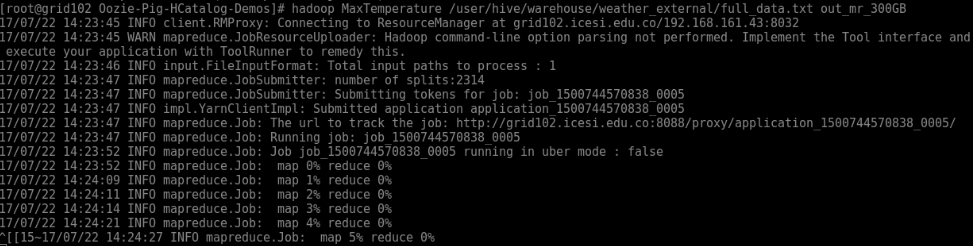
\includegraphics[width=\textwidth, height=1.5in]{fig/04/00}
  \caption{Monitoreo de la ejecución del programa \textit{MaxTemperature} en MapReduce por medio de la consola en donde éste se ejecutó.}
\end{figure}

\begin{figure}[H]
  \centering
      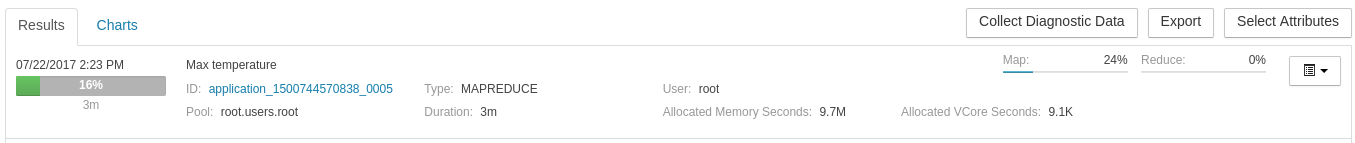
\includegraphics[width=\textwidth, height=1.0in]{fig/04/01}
  \caption{Monitoreo de la ejecución del programa \textit{MaxTemperature} en MapReduce por medio de la interfaz de YARN.}
\end{figure}

\begin{figure}[H]
  \centering
      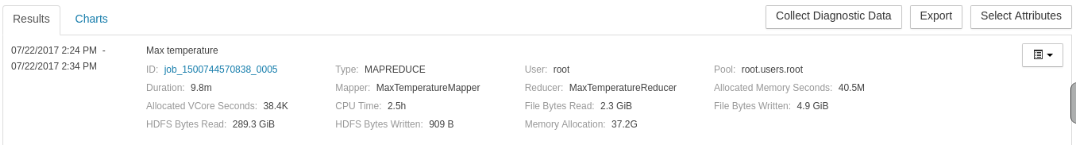
\includegraphics[width=\textwidth, height=1.0in]{fig/04/02}
  \caption{Ejecución finalizada.}
\end{figure}

\subsection{Ejecución con Hive}

A continuación se detallan los pasos necesarios para ejecutar el programa \textit{MaxTemperature} en su versión Apache Hive. \\

\subsubsection{Ejecución con la consola de Hive}

El siguiente script detalla la ejecución del programa \textit{MaxTemperature} en su versión Apache Hive.

\begin{lstlisting}[linewidth=\columnwidth,breaklines=true]
ADD jar /usr/lib/&hive&/lib/&hive&-contrib-1.1.0-cdh5.10.1.jar; 
INSERT OVERWRITE DIRECTORY 'out_max_hive_300GB' 
SELECT observation_date_year, MAX(air_temperature) 
FROM weather_managed 
WHERE air_temperature != 9999 AND at_quality_code IN (0,1,4,5,9) 
GROUP BY observation_date_year;
\end{lstlisting} 

\subsubsection{Seguimiento a la ejecución del programa}

El monitoreo de la ejecución del programa podrá realizarse a través de la interfaz gráfica de YARN, o por la información proporcionada por el Job History Server.

\begin{figure}[H]
  \centering
      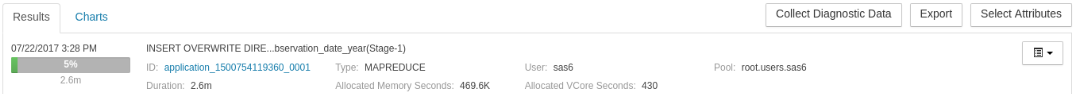
\includegraphics[width=\textwidth, height=0.6in]{fig/04/06}
  \caption{Monitoreo de la ejecución del programa \textit{MaxTemperature} en Hive por medio de la interfaz de YARN. }
\end{figure}

\begin{figure}[H]
  \centering
      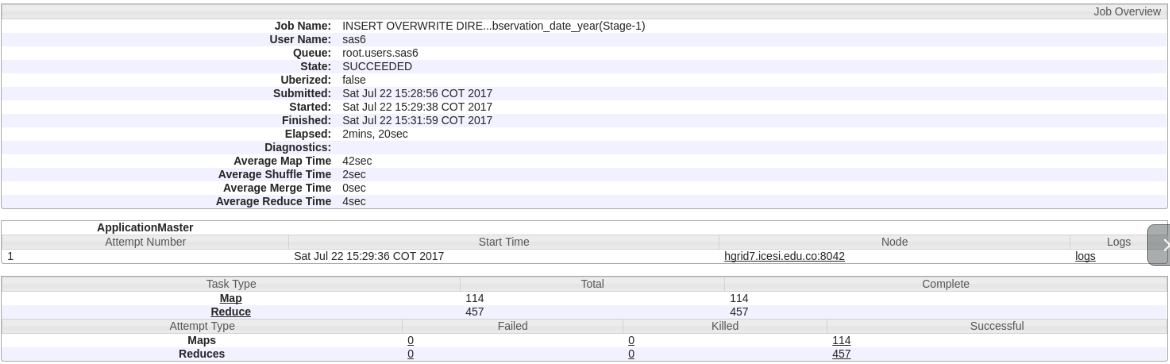
\includegraphics[width=\textwidth, height=2.5in]{fig/04/07}
  \caption{Ejecución finalizada, vista desde el Job History Server.}
\end{figure}


\subsection{Ejecución con Pig}

A continuación se detallan los pasos necesarios para ejecutar el programa \textit{MaxTemperature} en su versión Apache Pig. \\

\subsubsection{Definición del script en PigLatin}

El siguiente script contiene el código utilizado utilizado para ejecutar el programa \textit{MaxTemperature} en su versión PigLating. En las dos primeras lineas del script se detalla el uso de una UDF (\textit{User defined function}), provista por Tom White, para la lectura de registros a partir de la definición de rangos de lectura para sus atributos. El contenido del script fue guardado en un archivo llamado \textit{max-temp.pig}.

\begin{lstlisting}[linewidth=\columnwidth,breaklines=true]
REGISTER $load_loc;
records = LOAD '$in_s1' USING &com.hadoopbook.pig.CutLoadFunc&('16-19,88-92,93-93') AS (year:int, temperature:int, quality:int); 
filtered_records = FILTER records BY temperature != 9999 AND &com.hadoopbook.pig.IsGoodQuality&(quality);
grouped_records = GROUP filtered_records BY year;
max_temp = FOREACH grouped_records GENERATE group,MAX(filtered_records.temperature);
STORE max_temp INTO '$out_max';   
\end{lstlisting} 


\subsubsection{Definición de los parámetros del script}

Una vez definido el script en PigLatin, se procede a definir en un nuevo archivo los parámetros necesarios para la correcta ejecución del script. Los parámetros mencionados fueron guardados en un archivo llamado \textit{max.param}.

\begin{lstlisting}[linewidth=\columnwidth,breaklines=true]
# Load function location.
load_loc=/home/sas6/Oozie-Pig-HCatalog-Demos/assets/&pig&-examples.jar
# Input.
in_s1=/user/&hive&/warehouse/weather_external/full_data.txt
# Output.
out_max=out_max_pig
\end{lstlisting}

\subsubsection{Ejecución con Grunt en modo \textit{batch}}

A continuación se detalla el comando utilizado para ejecutar el programa \textit{MaxTemperature} mediante el modo \textit{batch} de Grunt.

\begin{lstlisting}[linewidth=\columnwidth,breaklines=true]
pig -param_file /home/sas6/Oozie-Pig-HCatalog-Demos/scripts/&pig&/300GB/max.param /home/sas6/Oozie-Pig-HCatalog-Demos/src/&pig&/max-temp.&pig&
\end{lstlisting}

\subsubsection{Seguimiento a la ejecución del programa}

El monitoreo de la ejecución del programa podrá realizarse a través de Grunt, por medio de la interfaz gráfica de YARN, o por la información proporcionada por el Job History Server.

\begin{figure}[H]
  \centering
      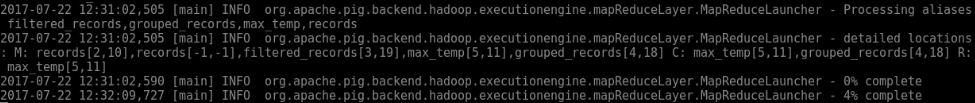
\includegraphics[width=\textwidth, height=1.0in]{fig/04/03}
  \caption{Monitoreo de la ejecución del programa \textit{MaxTemperature} en Pig por medio de la consola Grunt desde donde se ejecutó.}
\end{figure}

\begin{figure}[H]
  \centering
      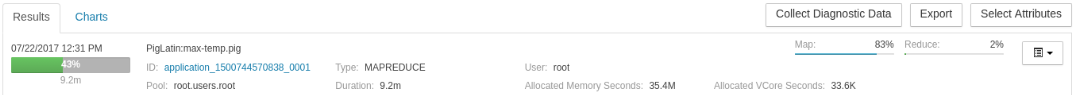
\includegraphics[width=\textwidth, height=0.6in]{fig/04/04}
  \caption{Monitoreo de la ejecución del programa \textit{MaxTemperature} en Pig por medio de la interfaz de YARN.}
\end{figure}

\begin{figure}[H]
  \centering
      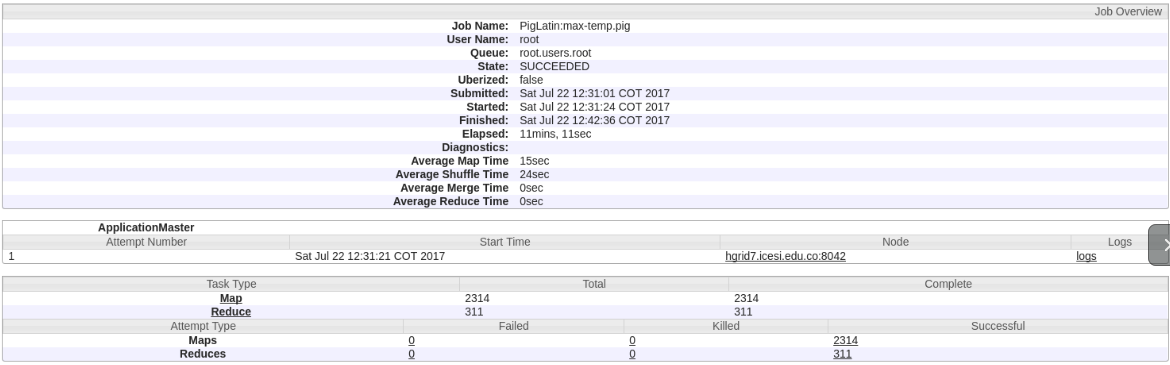
\includegraphics[width=\textwidth, height=2.5in]{fig/04/05}
  \caption{Ejecución finalizada, vista desde el Job History Server.}
\end{figure}

